\documentclass[a4paper, 12pt, english]{article}

% \usepackage[portuges]{babel}
\usepackage[utf8]{inputenc}
\usepackage{amsmath,amssymb}
\usepackage{graphicx}
\usepackage{subfig}
\usepackage[colorinlistoftodos]{todonotes}

\usepackage{indentfirst}
\usepackage{verbatim}
\usepackage{textcomp}
\usepackage{gensymb}

\usepackage{relsize}

\usepackage{lipsum}% http://ctan.org/pkg/lipsum
\usepackage{xcolor}% http://ctan.org/pkg/xcolor
\usepackage{xparse}% http://ctan.org/pkg/xparse
\NewDocumentCommand{\myrule}{O{1pt} O{2pt} O{black}}{%
  \par\nobreak % don't break a page here
  \kern\the\prevdepth % don't take into account the depth of the preceding line
  \kern#2 % space before the rule
  {\color{#3}\hrule height #1 width\hsize} % the rule
  \kern#2 % space after the rule
  \nointerlineskip % no additional space after the rule
}
\usepackage[section]{placeins}

\usepackage{booktabs}
\usepackage{colortbl}%
   \newcommand{\myrowcolour}{\rowcolor[gray]{0.925}}
   
\usepackage[obeyspaces]{url}
\usepackage{etoolbox}
\usepackage[colorlinks,citecolor=black,urlcolor=blue,bookmarks=false,hypertexnames=true]{hyperref} 

\usepackage{geometry}
\geometry{
	paper=a4paper, % Change to letterpaper for US letter
	inner=3cm, % Inner margin
	outer=3cm, % Outer margin
	bindingoffset=.5cm, % Binding offset
	top=2cm, % Top margin
	bottom=2cm, % Bottom margin
	%showframe, % Uncomment to show how the type block is set on the page
}
%*******************************************************************************%
%************************************START**************************************%
%*******************************************************************************%
\begin{document}

%************************************TITLE PAGE**************************************%
\begin{titlepage}
\begin{center}
\textbf{\LARGE Universidade Federal de Alagoas}\\[0.5cm] 
\textbf{\large Instituto de Computação - IC}\\[0.2cm]
\vspace{20pt}
%* \includegraphics{Logo_Utar.png}\\[1cm] *%

\par
\vspace{20pt}
\vspace{20pt}
\vspace{20pt}
\vspace{20pt}
\vspace{20pt}
\vspace{20pt}
\vspace{20pt}
\vspace{20pt}
\vspace{20pt}
\textbf{\Large Aluno: Marcos Gleysson Silva do Nascimento}\\ 
\vspace{15pt}
\myrule[1pt][7pt]
\textbf{\LARGE  Seminário 1}\\
\vspace{15pt}
\textbf{\large Análise e Classificação estatísticas para imagens SAR }\\
\myrule[1pt][7pt]
\vspace{25pt}
\textbf{\large Orientador: Alejandro Frery}\\

% 2. Low Hui Tyen \hspace{45pt} 14AGB06230 \\ % No2

\vspace{45pt}
\end{center}

\par
\vfill
\begin{center}
\textbf{Maceió - AL}\\
\textbf{2017}
\end{center}

\end{titlepage}

%************************************TABLE OF CONTENTS**************************************%

%  %Sumário
%  \newpage
%  \tableofcontents
%  \thispagestyle{empty}
%  %End Sumário

%********************************%
%***********SECTION 1************%
%********************************%
\newpage
\section{Introdução}
A intensificação de estudos na área de Sensoriamento Remoto voltado para os
radares imageadores de abertura sintética (Sinthetic Aperture Radar - SAR) tem
proporcionado, cada vez mais, o melhor entendimento dos mecanismos de dispersão dos
alvos terrestres na faixa de microondas. Desta forma, as aplicações de imagens SAR nos
mais variados campos do conhecimento humano (Geologia, Cartografia, etc.) tornam-se
mais confiáveis, principalmente em regiões onde a obtenção de imagens geradas por
sensores ópticos é muito difícil, devido a fatores climáticos.

Nesse sentido, o radar possui uma clara vantagem sobre sensores ópticos, devido
ao fato de sua capacidade ser praticamente inafetada pela escuridão, pelas nuvens ,
neblina e fumaça. O retroespalhamento do radar é muito sensível a vários parâmetros do
alvo e do sistema. Essa característica fornece informações multidimensionais que podem
ser usadas em áreas importantes como monitoramento agrícola, especialmente se um
radar de alta resolução, como no caso do SAR – Radar de Abertura Sintética – é utilizado.

Cada vez mais os algoritmos de classificação para imagens SAR tornam-se mais
precisos, quando os resultados por eles obtidos são comparados com verdades terrestres.
Essa melhora está diretamente ligada, entre outros fatores, a uma modelagem mais
adequada aos dados SAR, como mostrada em Nezry et al. (1996) e Frery et al. (1997).

Em Vieira (1996) isso fica bem evidente, através do uso das distribuições mais
apropriadas às observações (radiometria) provindas de diferentes classes, utilizadas na
classificação por Máxima Verossimilhança (MaxVer), além da modelagem das classes
(informação contextual) através do algoritmo Iterated Conditional Modes (ICM).

Com o advento de novos sensores, pode-se dispor cada vez mais de um grande
volume de imagens de sensoriamento remoto. Torna-se necessário, pois, processar-se
imagens de forma rápida e obter-se de maneira precisa a informação procurada. Uma das
técnicas mais úteis no processamento de imagens é a da classificação automática na qual
se permite automatizar tarefas associadas à interpretação visual de imagens, diminuindo
assim o tempo entre a aquisição dos dados e a sua análise.

Embora existam várias técnicas de classificação automática de imagens, poucas
delas são adequadas para os problemas particulares que apresentam as imagens SAR. A
maioria dos procedimentos para a análise e classificação de imagens disponíveis em
sistemas comerciais se baseia na hipótese de que os dados sejam normalmente
distribuídos, hipótese rara observada nas imagens SAR. As propriedades estatísticas das
imagens SAR dependem de parâmetros do sistema imageador como também de
parâmetros do alvo a ser imageado.

Verifica-se dessa forma a necessidade de se desenvolver técnicas e procedimentos
estatísticos específicos para análise e classificação de imagens SAR.

%********************************%
%***********SECTION 2************%
%********************************%
\newpage
\section{Modelos Estatísticos para dados SAR}
O modelo multiplicativo é comumente adotado para a explicação do comportamento
estatístico de dados obtidos com radiação coerente, como é o caso das imagens SAR. Este
modelo supõe que o valor observado em cada pixel é a ocorrência de uma variável aleatória Z = X.Y, onde X representa a variável aleatória referente ao retroespalhamento do pulso incidente na superfície terrestre (backscatter) e Y representa a variável aleatória referente ao ruído associado à radiação coerente (speckle). Diferentes distribuições para X e Y acarretam diferentes distribuições para a variável aleatória Z.

Nesse contexto decorre-se do Método Multiplicativo, a distribuição GA que possui
como casos especiais as seguintes distribuições: KA, GA0 e $\Gamma^{1/2}$. Observa-se a GA0 modela bem dados provenientes de áreas extremamente heterogêneas como é o caso de
áreas urbanas, enquanto que as distribuições KA e $\Gamma^{1/2}$. são utilizadas para modelagem de áreas heterogêneas (floresta) e homogêneas (solo exposto, pastagem, culturas agrícolas). O grau de homogeneidade está associado, entre outros fatores, aos parâmetros do sensor.

\subsection{SAR MONOESPECTRAL}
Para explicar o comportamento estatístico desse tipo de dado SAR, o modelo multiplicativo
é bastante empregado, pois tanto o backscatter como o speckle podem ser modelados de
formas diferentes, dependendo do tipo de aplicação (Yanasse, 1991; Yanasse et al., 1995;
Vieira, 1996; Frery et al., 1997). Dependendo dos diferentes tipos de detecção, linear
(imagem em amplitude) e quadrática (imagem em intensidade), e das diferentes regiões
imageadas, as distribuições associadas a X e Y variam, produzindo diferentes distribuições
para Z (Ulaby e Dobson, 1989; Frery et al., 1997). Distribuições decorrentes do modelo
multiplicativo para imagens SAR monoespectrais em intensidade possuem as variáveis
aleatórias X e Y , associadas a esse modelo com o subscrito “I”.

Sob certas condições (Ulaby et al, 1986; Goodman, 1963) pode-se supor que o speckle
possui uma distribuição G(n,n) , onde n é o número equivalente de looks3 (nel). Várias
distribuições podem ser utilizadas para o backscatter, visando a modelagem para diferentes
tipos de classes e seus diferentes graus de homogeneidade. Por exemplo, para alguns
parâmetros do sensor (comprimento de onda, ângulo de incidência, polarização, etc.) uma
pastagem pode ser mais homogênea que floresta, a qual é mais homogênea que áreas
urbanas.

Frery et al. (1997) apresenta a modelagem para o caso geral, considerando que
o backscatter possui uma distribuição Gaussiana Inversa Generalizada. Esta distribuição
possui casos especiais mais simples que têm se mostrado úteis na modelagem de áreas
com diferentes graus de homogeneidade. A modelagem para esses casos especiais possui
a vantagem de tornar mais fácil a estimação dos parâmetros das distribuições.

Na Figura 1 abaixo são apresentadas, para dados em intensidade multi-look (ou n-looks), as
possíveis distribuições associadas a regiões com diferentes graus de homogeneidade,
denominadas aqui de regiões homogêneas, heterogêneas e extremamente heterogêneas.

 \begin{figure}[!ht]
 			\begin{center}
				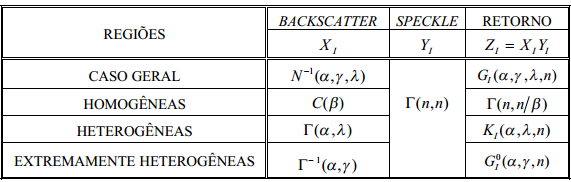
\includegraphics[width=100mm,scale=0.5]{tabela.png}
			\end{center}
       		\caption{\label{Retorno em intensidade para N - Looks}}
 \end{figure}

%********************************%
%***********SECTION 3************%
%********************************%

\section{Introdução a números pseudoaleatórios}

Numeros aleatórios perfazem uma das partes mais importantes em aplicações computacionais nos varios campos do conhecimento, como aborda [Knuth 1998]. Existem dois tipos básicos de geradores: Geradores de Números Aleatórios, do inglês Random Number Generators (RNGs) e Geradores de Numeros Pseudoaleat órios, do inglês Pseudorandom Number Generators (PRNGs). Computadores sao máquinas determinísticas e, portanto,
não e possível gerar sequencias aleatórias de forma algorítmica. Para construir RNGs utiliza-se uma fonte nao determinística de dados juntamente com algumas funções de 
processamento para produzir as sequências. A maior parte dos RNGs utiliza fenômenos físicos naturais como decaimento radioativo, ruídos térmicos em semicondutores, amostras de som em um local ruidoso, ruído no espectro eletromagnético, dentre outros; tais 
fontes de aleatoriedade não fazem parte do hardware usual de computadores. Como consequência, quando há necessidade de se dispor de dados que exibam aleatoriedade, lança-
se mão de PRNGs.

A maneira mais conveniente e confiável de se gerar números pseudoaleatórios em máquinas determinísticas é através de algoritmos que produzem sequências com comportamento semelhante as produzidas por RNGs. Tais algoritmos produzem sequências de 
numeros não aleatórios, mas que, sob certas condições, comportam-se como aleatórios. Como define [L’Ecuyer 2007], essas sequências podem ser chamadas pseudoaleatórias,
e os programas utilizados em sua produção de geradores de números pseudoaleatórios. Esses geradores sao geralmente mais convenientes do que os RNGs pois não necessitam de hardware adicional e possibilitam a reproducibilidade.

Os PRNGs sao a principal fonte de aleatoriede em jogos por computador, e no desenvolvimento de técnicas computacionais intensivas como os métodos Monte Carlo [Cipra 2000] e MCMC – Monte Carlo Markov Chain [Diaconis 2009].


%********************************%
%***********SECTION 4************%
%********************************%

\subsection{Principais técnicas de geração de número pseudo-aleatórios}

Os números pseudoaleatórios muitas vezes parecem ser mais aleatórios do que números
aleatórios obtidos de fontes físicas, pois se uma pseudo-sequência está bem construída,
cada valor na sequência é produzido a partir do valor anterior por meio de transformações
que parecem introduzir uma aleatoriedade adicional [Rukhin et al., 2010].

Segundo [Vieira et al., 2004], os tipos de geradores de números aleatórios e pseudoaleatórios
mais conhecidos e utilizados são:

\begin{itemize}

\item \textbf{Geradores Congruentes Lineares} [Press et al., 1992]: É um dos mais antigos e conhecidos
algoritmos para a criação de números aleatórios, sendo o número gerado pela fórmula:

\begin{equation}
	x_{n+1} = (ax_{n} + c) \quad \textit{mod} \quad  m, \qquad n >= 0
\end{equation}

onde, \begin{math} x_{n+1} \end{math} é o número gerado, \begin{math} x_{n} \end{math} é o número anterior, \begin{math} x_{0} \end{math} é a semente (que deve ser
fornecida por um RNG) e a, c e m são constantes.

\item \textbf{Geradores de Atraso de Fibonacci} [Marsaglia, 1985]: Tem-se esse nome por causa
similaridade com a sequência de Fiboncacci, sendo o número gerado pela fórmula:

\begin{equation}
x_{n} = x_{n-1} \quad op \quad x_{n-k}, \qquad 0<k<l
\end{equation}

onde \begin{math} x _{n} \end{math} é o número gerado e \textit{op} pode ser uma adição, subtração, multiplicação módulo m ou a operação \textit{ou exclusivo}.

\item \textbf{Geradores de Registradores de Deslocamento} [Marsaglia, 1985]: Consideram os bits
de uma palavra de computador como os elementos de um vetor binário, na qual,
iterativamente, através de transformações lineares
, geram sequências de vetores
binários interpretadas como sequências de números inteiros aleatórios uniformes.

\item \textbf{Geradores Híbridos} [Marsaglia, 1985]: É a combinação de dois ou mais geradores
com o objetivo de obter um gerador melhor.

\end{itemize}

\section{Projeto PIBIC}

O foco do meu projeto consiste em desenvolver técnicas de simulação e de estimação de parâmetros para distribuições de interesse na análise de imagens de radar de abertura sintética (Synthetic Aperture Radar — SAR). Essas
distribuições seguem o modelo multiplicativo, e suas ocorrências podem ser obtidas por diversas maneiras.
A estimação dos parâmetros dessas distribuições é, frequentemente, sujeita a instabilidades numéricas, viés
e alta variabilidade. Por esse motivo, a literatura discute diversas técnicas para construir estimadores (por 
analogia, máxima verossimilhança, e com kernels), bem como para melhorá-los (com robustez, reamostragem e modificações analíticas).

Minha frente de trabalho será desenvolvida na plataforma computacional R e como ferramenta para controle de versões será utilizado o Git. Especificamente o título do plano de trabalho é \textit{Desenvolvimento de Bibliotecas para Simulação e Inferência em Modelos para Imagens SAR} e o objetivo central do meu trabalho é implementar uma biblioteca de funções para a estimação de parâmetros de modelos para dados SAR.

Para verificar a qualidade numérica das funções implementadas será utilizado um protocolo próprio baseado em dados simulados. No tocante à robustez dos algoritmos, verificaremos o comportamento do sistema diante de possíveis problemas dos dados de entrada de modo deixar o \textit{software} produzido o mais robusto possível. Por fim para o desenvolvimento dos trabalhos será adotado uma versão do Modelo em Espiral do desenvolvimento de \textit{software}, adaptado às necessidades do \textit{software} científico.




\end{document}